\chapter{Plano de Continuidade}

Esta foi a primeira etapa do trabalho. Na próxima etapa, planeja-se: (1) propor uma combinação de ferramentas para o desenvolvimento de aplicações com arquitetura de microsserviços, (2) contextualizar essas ferramentas e apontar os problemas que elas resolvem, (3) desenvolver uma aplicação de exemplo com arquitetura de microsserviços usando as ferramentas propostas e boas práticas discutidas e (4) discutir pontos positivos e negativos das ferramentas usadas nessa aplicação de exemplo. O cronograma de atividades previstas para serem realizadas na disciplina de Trabalho de Conclusão de Curso 2 é apresentado na \autoref{figura-grafico-gantt}.

\begin{figure}[htb]
	\caption{\label{figura-grafico-gantt}Cronograma de atividades que serão desenvolvidas.}
	\begin{center}
	    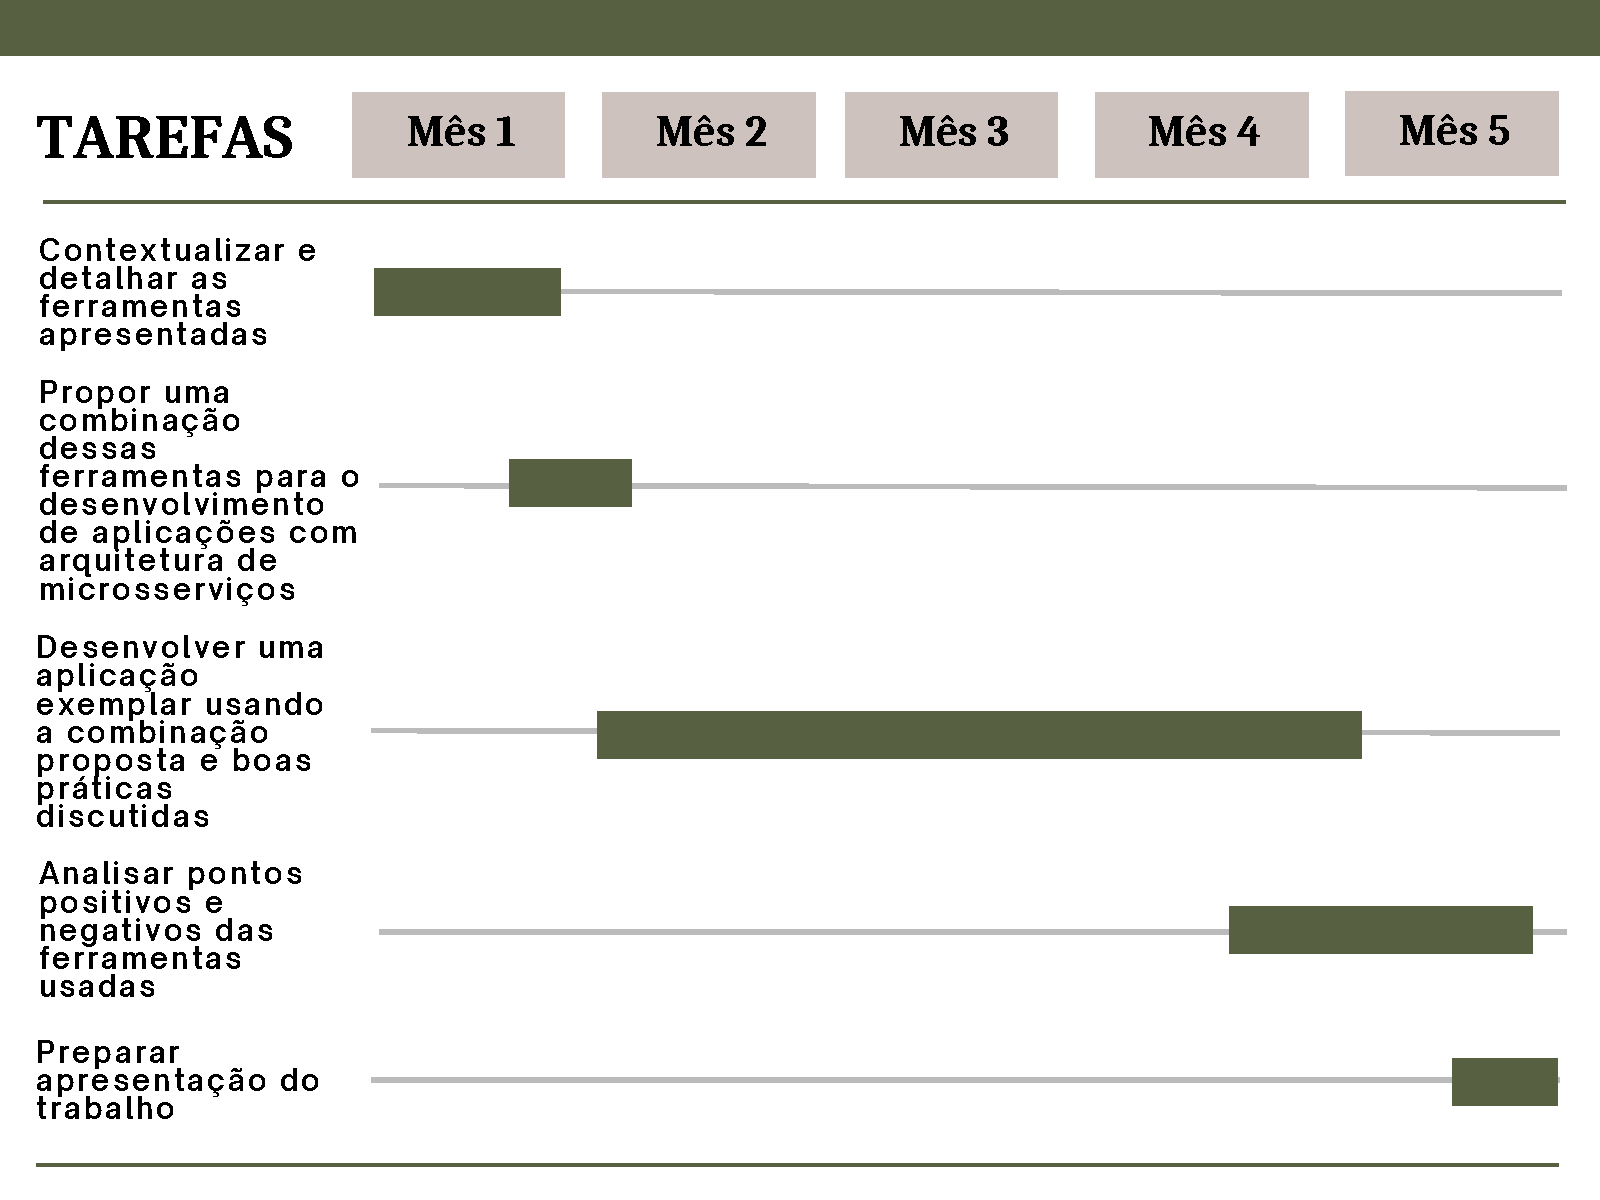
\includegraphics[scale=0.5]{Imagens/grafico-gantt.pdf}
	\end{center}
	\legend{Fonte: Autor}
\end{figure}
